\chapter{Введение}
\section{Глоссарий}
\begin{itemize}
  \item КА -- космический аппарат
  \item Апогей -- наиболее удаленная от одного из фокусов точка орбиты
  \item Перигей -- ближайшая к одному из фокусов точка орбиты
  \item Линия узлов -- линия пересечения плоскостей орбиты и экватора
  \item Узел орбиты -- следы линии узлов на небесной сфере
  \item Восходящий узел -- точка на небесной сфере, в которой спутник пересекает
  экватор в своем движении из южного полушария в северное
  \item Нисходящий узел -- узел, противоположный восходящему
  \item Долгота восходящего узла ($\Omega$) -- угол между направлениями на точку весеннего
  равноденствия и на восходящий узел
  \item Наклонение ($i$) -- угол между экваториальной плоскостью и плоскостью орбиты.
  \item Аргумент перигея ($\omega$) -- угловое расстояние от линии узлов в плоскости
  орбиты до направления на перигей орбиты
  \item Аргумент широты ($u$) -- угол, отсчитываемый в плоскости орбиты от линии
  узлов до текущего радиуса-вектора орбиты
  \item ОСК -- орбитальная система координат
\end{itemize}
\section{Описание предметной области}
\noindent\indent Идея создания солнечных парусов возникла ещё в начале XX в.
С того момента, как Максвелл теоретически обосновал, что излучение может создавать давление,
ученые задумались о том, как использовать давление солнца как движущую силу.\par
В 1924 Константином Цилковским и Фридрихом Цандером впервые был предложен концепт
использования такой конструкции, как солнечный парус, что позволяет использовать
такое явление, как солнечное давление на качественно новом уровне.\par
В 1974 эффект солнечного давления был впервые продемонстирован на движении межпланетного
космического аппарата Маринер 10. На солнечные панели Маринера 10 под различными углами к солнцу
действовало различное солнечное давление, что влияло на вращательное движение аппарата.\par
В конце 70-хх годов в NASA Jet Propultion Laboratory (JPL) активно стали изучать
возможность использования технологии солнечного паруса для подхода космических аппаратов
в близи комметы Галлея во время её попадания в 1986 в область Солнечной системы.\par
В виду большых затрат энергии для этой миссии, идея использования солнечного паруса
и энергии солнечного давления в целом выглядела весьма перспективной.
Однако, в то время разработки с использованием ионных двигателей были доработаны и составляли
большую конкуренцию солнечному парусу. В сентябре 1977 года в NASA отдали предпочтение
проекту на ионном двигателе, хотя позже и этот проект был свёрнут из-за недостатка финансирования.\par
Несмотря на то, что миссия к комете Галлея была свёрнута NASA, разработки солнечного паруса
породили значимый интерес к этой идее.
\section{Неформальная постановка задачи}
\noindent\indent Реализация математической модели управления КА в рамках данной
работы включает в себя следующие основные задачи:
\begin{enumerate}[label=\arabic*.]
  \item Разработка модуля по расчету результирующих сил и моментов, действующих
  на солнечный парус
  \item Реализация алгоритма поиска оптимального управления парусом
  \begin{enumerate}[label*=\arabic*.]
    \item Оптимальное управление в случае стационарной задачи
    \item Оптимальное управление в случае нестационарной задачи
  \end{enumerate}
  \item Интеграция разработанных решений с приложением <<Sputnix Satellite Simulator>>
\end{enumerate}
\section{Постановка задачи}
\subsection{Невозмущенное движение. Кеплеровы элементы орбиты}
\noindent\indent Движение спутника осуществляется в поле тяготения Земли. Основной силой,
действующей на небесное тело является сила всемирного тяготения: две материальные точки,
обладающие массами $m$ и $M$, тяготеют друг к другу с силой
\begin{equation} \label{eq:GForce}
  \vec{F} = G\frac{mM}{r^2},
\end{equation}
где $r$ -- расстояние между центрами тел, а $G$ -- универсальная постоянная тяготения
($G = 6.67\cdot10^{-8}\text{см}^3/г\cdot\text{сек}^2$).\par
Если рассматривать движение одного из тел (спутника) с массой $m$ относительно
другой (Земли) с массой $M$, считая, что можно пренебречь всеми силами, кроме силы
(\ref{eq:GForce}), то дифференциальные уравнения движения получат вид
\begin{equation}
  \begin{aligned}
    &\ddot{x} + \frac{\mu x}{r^3} = 0, \\
    &\ddot{y} + \frac{\mu y}{r^3} = 0, \\
    &\ddot{z} + \frac{\mu z}{r^3} = 0,
  \end{aligned}
\end{equation}
где $\mu = GM$, $x$, $y$, $z$ -- координаты точки (спутника) с массой $m$ в
поступательно перемещающейся системе координат с началом в точке (центре Земли)
с массой $M$; $r = \sqrt{x^2 + y^2 + z^2}$. В самом деле, здесь пренебрегаются
<<посторонние>> силы, действующие на точку c массой $m$. Но эти силы действуют,
и с их учетом уравнения
\begin{equation} \label{eq:GAccelerationModify}
  \begin{aligned}
    &\ddot{x} + \frac{\mu x}{r^3} = f_x, \\
    &\ddot{y} + \frac{\mu y}{r^3} = f_y, \\
    &\ddot{z} + \frac{\mu z}{r^3} = f_z,
  \end{aligned}
\end{equation}
где $f_x$, $f_y$, $f_z$ -- компоненты добавочных ускорений. Уравнения
(\ref{eq:GAccelerationModify}), вообще говоря, уже не интегрируются.\par
Спутник обладает ускорением ньютоновской силы тяготения,
\begin{equation}  \label{eq:GAcceleration}
  \vec{f} = - \frac{\mu}{r^2}\vec{e}_r,
\end{equation}
направленным к центру Земли. В формуле (\ref{eq:GAcceleration}) $\vec{e}_r$ --
единичный вектор по направлению от центра Земли к спутнику (который считаем материальной точкой).\par
Этому ускорению соотвествует силовая функция ньютановского центрального поля сил
\begin{equation}
  U = \mu/r,
\end{equation}
так что компоненты ускорения по осям $x$, $y$, $z$ неподвижной системы координат,
начало которой совпадает с центром Земли, будут равны
\begin{equation} \label{eq::GAccelerationAxis}
  f_x = -\frac{\partial U}{\partial x} = - \frac{\mu x}{r^3}, \\
  f_y = -\frac{\partial U}{\partial y} = - \frac{\mu y}{r^3}, \\
  f_z = -\frac{\partial U}{\partial z} = - \frac{\mu z}{r^3},
\end{equation}
а урванения движения (\ref{eq::GAccelerationAxis}) интегрируемы. Орбиты удовлетворяющие
этим уравнениям, назовем кеплеровыми.\par
Ссылаясь на книгу "Очерки о движении космических тел" под авторством В. В. Белецкого,
известно, что спутник движется по эллиптической, параболической или гиперболической орбите,
такой, что с центром Земли совпадает фокус эллипса, параболы или гиперболы.\par
Нас будет интересовать в основном случай эллиптических орбит. На рис. \ref{fig:KeplerOrbit2D}
изображена такая орбита. В полярных координатах $r$, $\nu$ уравнение эллипса имеет вид
\begin{equation} \label{eq:GRENu}
  r = \frac{p}{1 + e\cos\nu}
\end{equation}
причем угол $\nu$ отсчитывается от направления $r_{\pi}$ из центра Земли к перигею.
\begin{wrapfigure}{r}{0.35\textwidth}
  \centering
  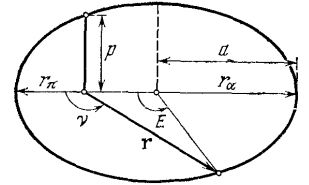
\includegraphics[width=0.35\textwidth]{Orbit_2D}
  \caption{Кеплеровская эллиптическая орбита}
  \label{fig:KeplerOrbit2D}
\end{wrapfigure}
Наибольшее удаление $r_{\alpha}$ спутника от Земли достигается в апогее при значении
$\nu = 180^{o}$. В уравнении (\ref{eq:GRENu}) величины $p$ и $e$ постоянны; $p$ называется
фокальным параметром орбиты, и его геометрический смысл ясен из рис. \ref{fig:KeplerOrbit2D};
эта величина характеризует размер орбиты; вторая величина -- эксцентриситет орбиты $e$ --
характеризует её сжатие, вытянутость. При $e = 0$ орбита круговая, а при $e \rightarrow 1$
орбита стремится к параболической. Величины $p$ и $e$ можно выразить через апогейное
($r_{\alpha}$) и перигеное ($r_{\pi}$) расстояния:
\begin{equation}
  p = \frac{2r_{\alpha}r_{\pi}}{r_{\alpha} + r_{\pi}},
  e = \frac{r_{\alpha} - r_{\pi}}{r_{\alpha} + r_{\pi}}.
\end{equation}
Наибольший размер эллипса характеризуется его большой полуосью $a$, при этом
\begin{equation}
  a = \frac{1}{2}(r_{\alpha} + r_{\pi}),
\end{equation}
а между $p$, $e$, $a$ существует связь
\begin{equation}
  p = a(1 - e^2).
\end{equation}
Угол $\nu$ в формуле \label{eq:GRENu} называется истинной аномалией.\par
Зависимость $\nu(t)$ от времени дает закон движения спутника по орбите. В теории
кеплеровских орбит наиболее трудное место -- отыскание явного выражения через время
$t$. Угловая скорость $d\nu/dt$ движения по орбите удовлетворяет так называемому
интегралу (или закону) площадей
\begin{equation} \label{eq:GIntegralSquares}
  r^2\frac{d\nu}{dt} = \sqrt{\mu p}.
\end{equation}\par
Если сюда подставить выражение $r(\nu)$ из (\ref{eq:GRENu}) и вычислить соответсвуюющую
квадратуру, то получим явное выражение времени через $\nu: t = t(\nu)$. Задача состоит
в решении этого трансцендентного уравнения относительно $\nu$. Для этого вводится
новая переменная $E$, называемая эксцентрической аномалией (смысл ее виден на том
же рис. \ref{fig:KeplerOrbit2D}) и связанная с $\nu$ соотношениями
\begin{equation}
  \cos\nu = \frac{\cos E - e}{1 - e\cos E}, \sin\nu = \frac{\sin E}{1 - e\cos E}\sqrt{1 - e^2},
\end{equation}
причем
\begin{equation}
  r = a(1 - e\sin E).
\end{equation}
Эксцентрическая аномалия $E$ связана со временем уравнением Кеплера:
\begin{equation} \label{eq:EscentricAnomaly}
  E - e\sin E = n(t-\tau^*),
\end{equation}
где $n = \sqrt{\mu/a^3}$ -- так называемое среднее движение; постоянная $\tau^*$
обозначает момент прохождения через перигей орбиты. Из (\ref{eq:EscentricAnomaly})
следует, что период обращения спутника по орбите
\begin{equation}
  T = 2\pi\sqrt{a^3/\mu}.
\end{equation}\par
Уравнение (\ref{eq:EscentricAnomaly}) не решается аналитически, поэтому для её
вычисления будем использовать один из алгоритмов численного решения уравнений, к примеру,
метод Эйлера:
\begin{equation}
  \begin{aligned}
    & E_{k+1} = e\sin E_k + M, \\
    & M = n(t - \tau^*).
  \end{aligned}
\end{equation}\par
Тем самым, положение спутника в каждый момент времени в плоскости орбиты
будет вычисляться по формуле:
\begin{equation}
  \begin{aligned}
    & \vec{r}_{orbital} = r \cdot [\cos\nu, \sin\nu, 0]^{T}, \\
    & r = a(1 - e\sin E)
  \end{aligned}
\end{equation}\par
Совершим переход из движения в плоскости орбиты к движению в пространстве, определив
компоненты фиксирующие положение орбиты в нем.
\begin{wrapfigure}{r}{0.35\textwidth}
  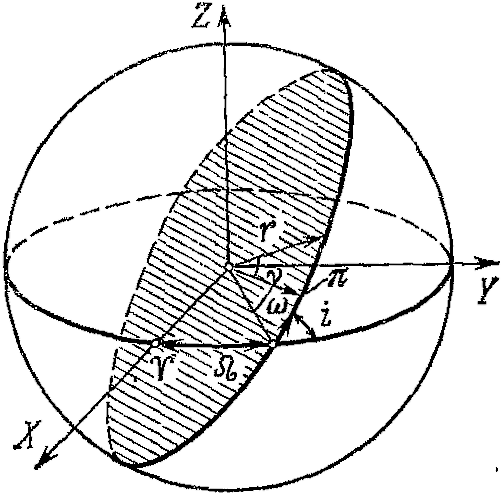
\includegraphics[width=\linewidth]{Orbit_Kepler.png}
  \caption{Кеплеровы элементы}
  \label{fig:KeplerOrbitParameters}
\end{wrapfigure}
Это положение описывают следующим образом (рис. \ref{fig:KeplerOrbitParameters}).
Спроектируем плоскость орбиты на небесную сферу и рассмотрим систему координат $XYZ$
такую, что ось $Z$ направлена на Северный полюс мира (вполне определенная точка
на небесной сфере вблизи Полярной звезды), ось $X$ -- на точку весеннего
равноденствия (тоже вполне определенная точка); начало координат совпадает с
центром Земли, а плоскость $XY$ -- с плоскостью земного экватора.
Вводятся такие переменные, как долгота восходящего узла ($\Omega$), наклонение ($i$),
аргумент перигея ($\omega$).\par
Обобщив это, получим, что орбита спутника характеризуется двумя независимыми постоянными
параметрами: $p$ и $e$; положение орбиты в пространстве определеяется тремя независимыми
углами: $\Omega$, $\omega$, $i$; положение спутника на орбите в каждый момент времени
определяется параметром $\tau^*$. Итак, имеем шесть независимых параметров, полностью
определяющих движение спутника в пространстве (его координаты и скорость в каждый
момент времени), например:
\begin{equation} \label{eq:KeplerOrbitalElements}
  p,\,\, e,\,\, \Omega,\,\, \omega,\,\, i,\,\, \tau^*
\end{equation}
Параметры (\ref{eq:KeplerOrbitalElements}) называются кеплеровыми элементами
орбиты спутника.
И положение спутника в пространстве в каждый момент времени будет вычисляться по формуле:
\begin{equation}
  \begin{aligned}
    & \vec{r} = R_z(\omega)R_x(i)R_z(\Omega) \cdot \vec{r}_{orbital}, \\
    & \vec{r}_{orbital} = r \cdot [\cos\nu, \sin\nu, 0]^{T}, \\
    & r = a(1 - e\sin E),
  \end{aligned}
\end{equation}\par
где $R_x$, $R_z$ -- матрицы поворота, выраженные следующим образом:
\begin{equation}
  \begin{aligned}
    & R_x(\phi) = \begin{bmatrix}
       1        &  0        &   0        \\
       0        &  \cos\phi &  -\sin\phi \\
       0        &  \sin\phi &   \cos\phi
    \end{bmatrix}, \\
    & R_y(\phi) = \begin{bmatrix}
       \cos\phi &  0        &  \sin\phi \\
       0        &  1        &  0        \\
      -\sin\phi &  0        &  \cos\phi
    \end{bmatrix}, \\
    & R_z(\phi) = \begin{bmatrix}
      \cos\phi & -\sin\phi & 0 \\
      \sin\phi &  \cos\phi & 0 \\
      0        &  0        & 1
    \end{bmatrix}.
  \end{aligned}
\end{equation}

\subsection{Возмущенное движение. Оскулирующие элементы}
\noindent\indent Кеплеровское движение, рассмотренное в предыдущем пункте, называют
ещё невозмущенным движением спутника. На самом же деле, при движении спутника под
действием возмущающих сил, кеплеровы элементы орбиты перестают быть постоянными,
и меняются со временем:
\begin{equation} \label{eq:KeplerOrbitalElementsTime}
  p(t),\,\, e(t),\,\, \Omega(t),\,\, \omega(t),\,\, i(t),\,\, \tau^*(t).
\end{equation}\par
Задача сводится тогда к отысканию явных зависимостей (\ref{eq:KeplerOrbitalElementsTime})
от времени.\par
<<Эллипс>> с переменными элементами (\ref{eq:KeplerOrbitalElementsTime}) называется
оскулирующим эллипсом, а сами переменные элементы -- оскулирующими элементами.\par
Чтобы составить дифференциальные уравнения для оскулирующих элементов (\ref{eq:KeplerOrbitalElementsTime}),
надо перейти от переменных $x$, $y$, $z$, $\dot{x}$, $\dot{y}$, $\dot{z}$ к переменным
(\ref{eq:KeplerOrbitalElementsTime}), подставить в уравнения (\ref{eq:GAccelerationModify})
и разрешить их относительно производных $\frac{dp}{dt}$, $\frac{de}{dt}$, $\frac{d\Omega}{dt}$,
$\frac{d\omega}{dt}$, $\frac{di}{dt}$, $\frac{d\tau^*}{dt}$ оскулирующих элементов.
\subsection{Уравнения в оскулирующих элементах}
\noindent\indent Ссылаясь на уже упомянутый труд В. В. Белецкого, приведем систему уравнений
в оскулирующих элементах орбиты:
\begin{equation}
  \begin{cases}
    \frac{dp}{dt} = 2r\sqrt{\frac{p}{\mu}}T, \\
    \frac{de}{dt} = \sqrt{\frac{p}{\mu}}\left\{
      S\sin\nu + T\left[(1 + \frac{r}{p})\cos\nu + e\frac{r}{p}\right]
    \right\}, \\
    \frac{d\omega}{dt} = \frac{1}{e}\sqrt{\frac{p}{\mu}}\left[
      -S\cos\nu + T(1 + \frac{r}{p})\sin\nu - W e\frac{r}{p}\sin u\ctg i
    \right] \\
    \frac{di}{dt} = W \frac{r}{\sqrt{\mu p}}\cos u, \\
    \frac{d\Omega}{dt} = W \frac{r}{\sqrt{\mu p}}\frac{\sin u}{\sin i}, \\
    \frac{d\tau^*}{dt} = \frac{r^2}{e\mu}\left[
      S (eN\sin\nu - \cos\nu) + T N\frac{p}{r}
    \right].
  \end{cases}
\end{equation}\par
\begin{figure}[h]
  \centering
  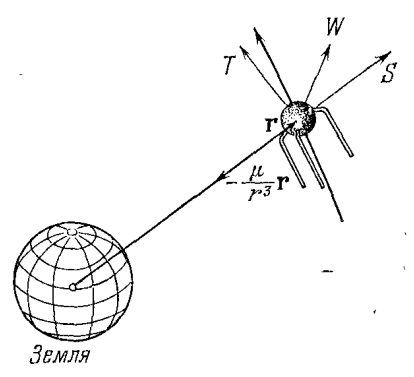
\includegraphics[width=0.35\textwidth]{ForcesOrientation}
  \caption{Система координат}
  \label{fig:ForcesOrientation}
\end{figure}\par
Здесь
\begin{equation}
  N = \frac{p^2}{r^2}\int\limits_0^{\nu} \frac{2\cos\nu}{(1 + e\cos\nu)^3}d\nu,\,\,
  u = \nu + \omega,
\end{equation}
и $S$, $T$, $W$ -- соответственно радиальное, трансверсальное и нормальное возмущающие
ускорения.\par
\subsection{Возмущения от зональных гармоник}
\noindent\indent Сила ньютоновского притяжения и соотвествующая силовая функция
лишь приближенно описывают силу притяжения, действующую на спутник со стороны
реальной Земли. Однако, в виду <<сплюснутости>> в направлении полюсов (и в малой
степени также и <<с боков>>), не совсем симметрична, неоднородна, в результате
чего поле сил, создаваемое Землей, имеет довольно сложную структуру. Для более
хорошего приближения к реальному полю сил представляют силовую функцию в следующем виде:
\begin{equation} \label{eq:UModifiy}
  U = \frac{\mu}{r}\left\{1 + \sum\limits_{k=2}^{\infty}I_k\left(\frac{R}{r}\right)^kP_k(\sin\phi)\right\},\,\,
  \mu = GM.
\end{equation}
Здесь $M$ -- масса Земли, $G$ -- универсальная постоянная тяготения, $R$ -- экваториальный
радиус Земли, $\phi$ -- географическая широта точки (отстоящей от центра Земли на
расстоянии $r$). Коэффициенты $I_k$ имеют фиксированные безразмерные значения.
Функции $P_k$ представляют собой полиномы Лежандра, определяемые следующим образом:
\begin{equation}
  \begin{cases}
    \begin{aligned}
      & P_0(x) = 1, \\
      & P_1(x) = x, \\
      & P_2(x) = \frac{1}{2}(3x^2 - 1), \\
      & P_3(x) = \frac{1}{2}(5x^3 - 3x), \\
      & ...\\
      & P_n(x) = \frac{1}{2^n \cdot n!}\frac{d^n}{dx^n}(x^2 - 1)^n, \\
    \end{aligned}
  \end{cases}
\end{equation}\par
Таким образом, силовая функция (\ref{eq:UModifiy}) зависит только от расстояния
до центра притяжения, как силовая функция, но ещё и от широты места. Силовая
функция предполагает, что поле сил осесимметрично (относительно оси, проходящей
через полюсы Земли). Видим, что (\ref{eq:UModifiy}) представляет собой сумму
ньютоновского потенциала и добавочных членов, которые, по определению возмущений,
должны быть малы по сравнению с основным (первым) членом. Действительно,
коэффициенты $I_k$ в (\ref{eq:UModifiy}) имют такие значения:
\begin{equation}
  \begin{cases}
    \begin{aligned}
      & I_2 = -1082.2\cdot10^{-6}, \\
      & I_3 = 2.3\cdot10^{-6}, \\
      & I_4 = 2.1\cdot10^{-6}, \\
      & ...,
    \end{aligned}
  \end{cases}
\end{equation}
так что даже самый большой из этих коэффициентов $I_2$ дает добавку порядка
десятой доли процента, а остальные коэффициенты -- ещё на несколько порядков
меньше. Коэффициент $I_2$ характеризует наиболее существенное отличие поля
тяготения реальной Земли от идеальной шаровой.\par
Рассмотрим влияние основного возмущения на движение спутника в поле тяготения Земли.
Итак, возмущающая силовая функция
\begin{equation}
  U = \frac{\mu}{r}I_2\left(\frac{R}{r}\right)^2 \frac{1}{2}(3\sin^2\phi - 1).
\end{equation}\par
  Для записи возмущающего ускорения, вызванного нецентральностью гравитационного
поля Земли, на оси орбитальной системы координат воспользуемся соотношениями,
вытекающими из рис. \ref{fig:GarmonicOrbitalEq}.\par
  На этом рисунке положение спутника характеризуется точкой A; плоскость орбиты
спутника есть EAF; меридиональная плоскость, проходящая через точку A, - BCD.
Угол между местным меридианом и трансверсальным направлением в точку A обозначен
$\psi$, угол ECA - $u$ (аргумент широты), угол ABC -- $\phi$ -- широта точки.
\begin{figure}[h]
  \centering
  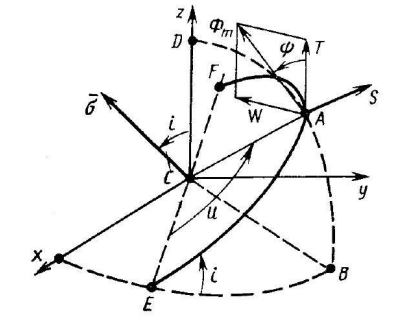
\includegraphics[width=0.35\textwidth]{GarmonicOrbitalEq}
  \caption{Проекции возмущающих ускорений в орбитальной системе координат}
  \label{fig:GarmonicOrbitalEq}
\end{figure}\par
Легко получить соотношения (\ref{eq:GarmonicOrbitalAcceleration}):\par
\begin{equation} \label{eq:GarmonicOrbitalAcceleration}
  \begin{aligned}
    & S = \frac{3I_2\mu R^2}{2r^4} \cdot (3\sin^2\phi - 1) = \frac{3I_2\mu R^2}{2r^4} \cdot (3\sin^2 i\sin^2 u - 1), \\
    & T = \frac{3I_2\mu R^2}{2r^4} \cdot (\sin2\phi\cos\psi) = - \frac{3I_2\mu R^2}{2r^4} \cdot (\sin^2 i\sin2 u), \\
    & W = \frac{3I_2\mu R^2}{2r^4} \cdot (\sin2\phi\sin\psi) = -\frac{3I_2\mu R^2}{2r^4} \cdot (\sin2 i\sin u), \\
  \end{aligned}
\end{equation}\par
При выводе последних равенств были использованы следующие формулы сферической
тригонометрии:
\begin{equation}
  \sin\phi = \sin u \sin i,\,\, \cos\psi = \ctg u \tg\phi,
\end{equation}
где $i$ -- наклонение орбиты, $u$ -- аргумент широты.
\subsection{Давление солнечного света}
\noindent\indent Сила светового давления включает в себя несколько составляющих:
давление от поглощенного излучения, отраженного, пропущенного, а также собственное
излучение паруса. Данные факторы зависят от соответсвующих оптимческих характеристик --
коэффициентов поглощения, отражения, пропускания и излучательной способности. В
общем случае данные факторы зависят от направления в пространстве, свойств поверхности,
длины волны, температуры поверхности и др.\par
  Предполагая начальную (раскройную) форму поверхности солнечного паруса плоской,
введем прямоугольную декартову систему координат $Ox_1x_2x_3$ на раскройной форме
солнечного паруса (рис. \ref{fig:SailCoordinateSystem}). Деформированное состояние
паруса зададим через поле векторов перемещения точек полотна паруса
$\vec{u} = (u_1, u_2, u_3)^T$. Зададим единичный вектор нормали $\vec{n}$,
положительное направление которого определено для освещенной стороны полотна паруса.
\begin{figure}[h]
  \centering
  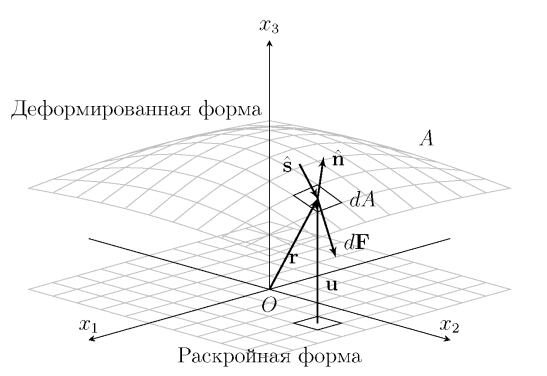
\includegraphics[width=0.5\textwidth]{SailCoordinateSystem}
  \caption{Раскройная форма солнечного паруса}
  \label{fig:SailCoordinateSystem}
\end{figure}
Определим единичный вектор $\vec{s}$, направленный от источника света на полотно
паруса. На достаточно большом удалении от Солнца вектор $\vec{s}$ можно считать
постоянным для всей поверхности солнечного паруса.\par
  Запишем элементарную силу светового давления как
\begin{equation}
  d\vec{F} = P(R) \cdot \left[
    -a_{10}(\vec{n}\cdot\vec{s})\vec{s}
    +a_{20}(\vec{n}\cdot\vec{s})\vec{n}
    -2a_{30}(\vec{n}\cdot\vec{s})^2\vec{n}
  \right]dA,
\end{equation}
здесь
\begin{equation}
  P(R) = \frac{q_0(R)}{c},
\end{equation}
-- световое давление ($q_0(R)$ -- солнечная постоянная, которая зависит от
расстояния $R$ до Солнца, $c$ -- скорость света в вакууме); $a_{10}$, $a_{20}$,
$a_{30}$ -- обобщенные оптические параметры, определяемые следующим образом:
\begin{equation}
  \begin{aligned}
    & a_{10} = 1 - \rho s, \\
    & a_{20} = B_f\rho(1 - s) + (1 - \rho)\frac{\epsilon_f B_f - \epsilon_b B_b}{\epsilon_f + \epsilon_b}, \\
    & a_{30} = \rho s, \\
  \end{aligned}
\end{equation}
причем $\rho$ -- коэффициент зеркального отражения; $s$ -- коэффициент зеркальности;
$B_f$ и $B_b$ -- коэффициенты, показывающие характер индикатрисы отражения за вычетом
зеркальной составляющей (в случае диффузного отражения $B = 2/3$); $e_f$ и $e_b$ --
излучательная способность освещенной и обратной сторон паруса.\par
  Параметры $a_{10}$ и $a_{30}$ учитывают зеркальную составляющую, а первое слагаемое
параметра $a_{20}$ в случае, когда $B_f$ и $B_b = 2/3$, -- диффузную составляющую.
Второе слагаемое параметра $a_{20}$ отвечает за вклад собственного теплового излучения
полотна в результирующую силу светового давления.\par
  Аналогично запишем выражения для момента от элементарной силы светового давления
\begin{equation}
  d\vec{M} = \vec{r} \times d\vec{F} = P(R) \cdot \left[
    -a_{10}(\vec{n}\cdot\vec{s})(\vec{r} \times \vec{s})
    +a_{20}(\vec{n}\cdot\vec{s})(\vec{r} \times \vec{n})
    -2a_{30}(\vec{n}\cdot\vec{s})^2(\vec{r} \times \vec{n})
  \right]dA,
\end{equation}
где $\vec{r}$ -- вектор, задающий положение элементаронй площадки $dA$.\par
  Векторы $\vec{s}$ и $\vec{n}$ задаются в ОСК выражениями\par
\begin{equation} \label{eq:SunVector}
  \vec{s} = \begin{bmatrix}
     \sin\psi_s\sin\theta_s \\
    -\cos\psi_s\sin\theta_s \\
     \cos\theta_s
  \end{bmatrix},
\end{equation}
\begin{equation}
  \vec{n} = \begin{bmatrix}
     \sin\psi\sin\theta \\
    -\cos\psi\sin\theta \\
     \cos\theta
  \end{bmatrix}.
\end{equation}\par
Связь компонент вектора Солнца $\vec{s}$ с положением плоскости орбиты относительно
направления на Солнце выявляется из сравнения (\ref{eq:SunVector}) и альтернативного
выражения
\begin{equation}
  \vec{s} = \begin{bmatrix}
    \sigma_x\cos u + \sigma_y\sin u \\
    \sigma_y\cos u - \sigma_x\sin u \\
    \sigma_z
  \end{bmatrix}
\end{equation}
через компоненты вектора $\sigma$, связанные с долготой восходящего узла $\Omega$,
наклонением $i$ и эклиптической долготой $\lambda$ по формуле
\begin{equation}
  \vec{\sigma} = R_x(-i)R_z(\Omega)R_x(\epsilon)R_z(\lambda)\vec{e}_x,
\end{equation}
где $\epsilon = 23^o26'$ -- наклон эклиптики к экватору. Имеем:
\begin{equation}
  \begin{aligned}
    & \theta_s = \arccos\sigma_z, \\
    & \psi_s = atan2(\sigma_x\cos u + \sigma_y\sin u, \sigma_x\sin u - \sigma_y\cos u).
  \end{aligned}
\end{equation}
Функция $atan2$ обозначает операцию взятия обратного тангенса с учетом знаков
обоих аргументов.
% \section{Математические методы}
% \subsection{}
\section{Обзор существующих решений}
\noindent\indent Рассмотрим некоторые существующие решения программ для моделирования
процесса управления солнечным парусом.
\subsection{<<GMAT>>}
\noindent\indent GMAT (General Mission Analysis Tool) -- ПО для решения задач связанных
с подготовкой космический миссий, оптимизации и навигации. Система используется для
моделирования как низкоорбитальных операций, так и операции в условиях нахождения
в глубоком космосе.
\subsection{<<Orekit>>}
\noindent\indent Orekit -- библиотека для работы с элементами небесной механики.
Данная библиотека предоставляет возможность использования готовых инструментов по расчету
действующих на аппарат возмущающих сил, включая рассчет вектора силы солнечного давления
действующего на КА.
\subsection{<<SaVoir>>}
\noindent\indent SaVoir -- планировщик движения нескольких спутников. Программное
решение, первоначально разработанное для европейского космического агенства
(<<the European Space Agency>>) с целью поддрежки операций в рамках международной
Хартии по космосу и крупным катастрофам.
\subsection{Сравнение основных характеристик}
\begin{tabular}{|l|c|c|c|}
  \hline
  Признак                      & GMAT                            & Orekit              & SaVoir \\ \hline
  Оптимизация управления       & +                               & +                   & +      \\ \hline
  Расчет сопротивления воздуха & +                               & +                   & +      \\ \hline
  Расчет солнечного давления   & +                               & +                   & -      \\ \hline
  Открытый исходный код        & +                               & +                   & -      \\ \hline
  Язык реализации              & C++                             & Java                & -      \\ \hline
  Лицензия                     & NOSA v1.3 & Apache License v2.0 & Проприетарная \\ \hline
\end{tabular}\par
Таким образом, учитывая требования к программному решению, принято решение
ориентироваться на программное решение GMAT во время разработки модулей для целевой программы.
